\newpage
\vspace{-6mm}
\section{}
실험 2에서는 SimuLTE를 통해 단말이 이동함에 따라 통신을 유지하면서 연결된 LTE 기지국(eNodeB) 바꾸는 handover 시뮬레이션을 진행한다.
\subsection*{Experiment 2-1}
    \subsubsection*{2. 1. 1 Code}
    \vspace{-3mm}
            \vspace{-2mm}
            \begin{listing}[h!]
            \inputminted[framerule = 1pt,framesep = 2mm , frame = lines, fontsize=\footnotesize]{c}{./code/week11/Experiment_02/omnet3.cpp}
            \vspace{-3mm}
            \caption{\footnotesize experiment 2-1, omnetpp.ini}
            \end{listing}
            \vspace{-6mm}
    \subsubsection*{2. 1. 2 Simulation}
    \vspace{-3mm}
        omnetpp.ini 파일을 실행시켜 다음과 같은 network를 build 했다. 두 개의 eNodeB, eNodeB1과 eNodeB2가 떨어져 위치해있고, 두 개의 단말 ue11과 ue12가  eNodeB1의 왼쪽에서  eNodeB2의 오른쪽을 직선으로 왕복한다. \\
        시뮬레이션 진행중 단말의 이동이 나타나도록 화면녹화 screenshot 영상을 촬영해 youtube에 업로드하였다. 해당 영상은 아래의 링크를 클릭해 이동이 가능하다.
        \vspace{-10mm}
            \begin{center}
                \item \href{https://www.youtube.com/watch?v=3oapMWzXq54&ab_channel=anamnesis}
            	{Youtube link of Week11 Experiment 2-1 Simulation Results Screenshot Video}
            \end{center}
        \vspace{-6mm}
        \begin{figure}[h!]
            \centering
            \subfloat[screenshot 1]{
                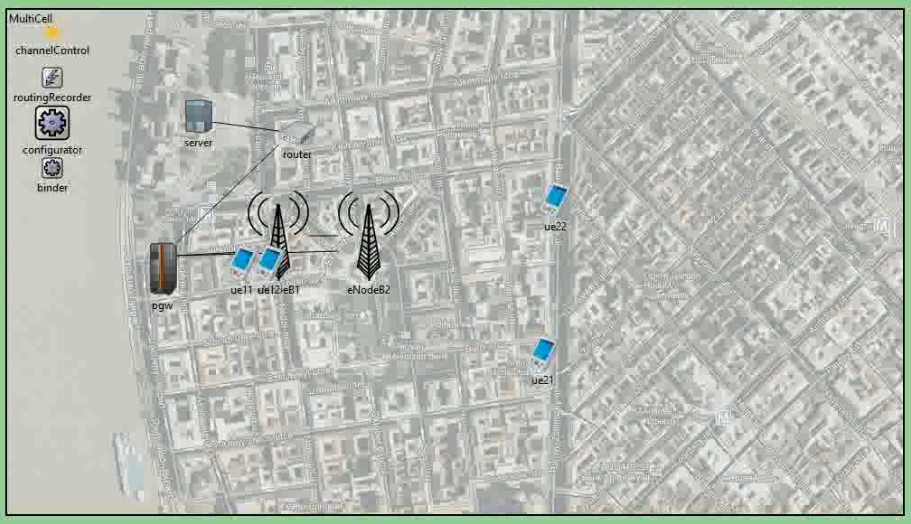
\includegraphics[width=0.45\textwidth]{image/week11/2-1-1.png}
            }\hspace{3mm}
            \subfloat[screenshot 2]{
                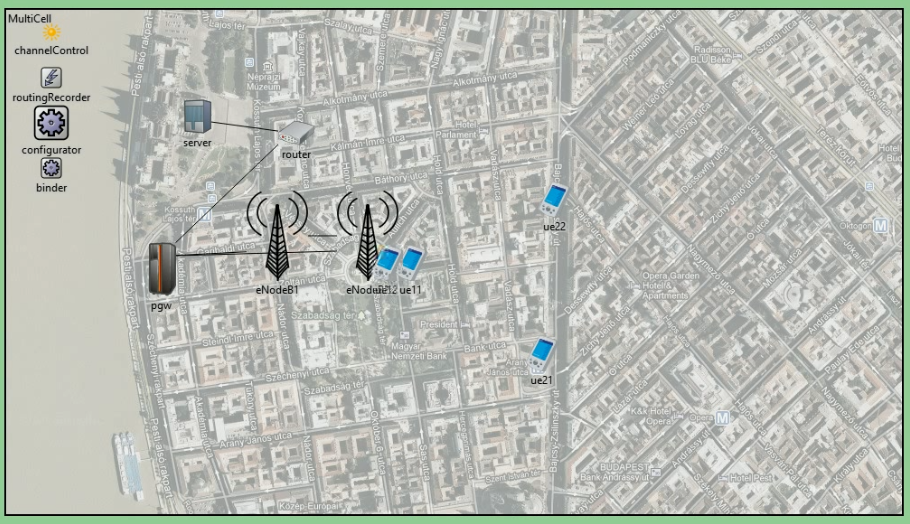
\includegraphics[width=0.45\textwidth]{image/week11/2-1-2.png}
            }\hspace{3mm}
            \caption{experiment 2-1, network simulation}
        \end{figure}
        시뮬레이션 종료 후 생성된 벡터 데이터 중에서 시간에 따른 단말 ue11의 servingCell 값을 확인했다.
        \begin{figure}[!h]\centering 
	        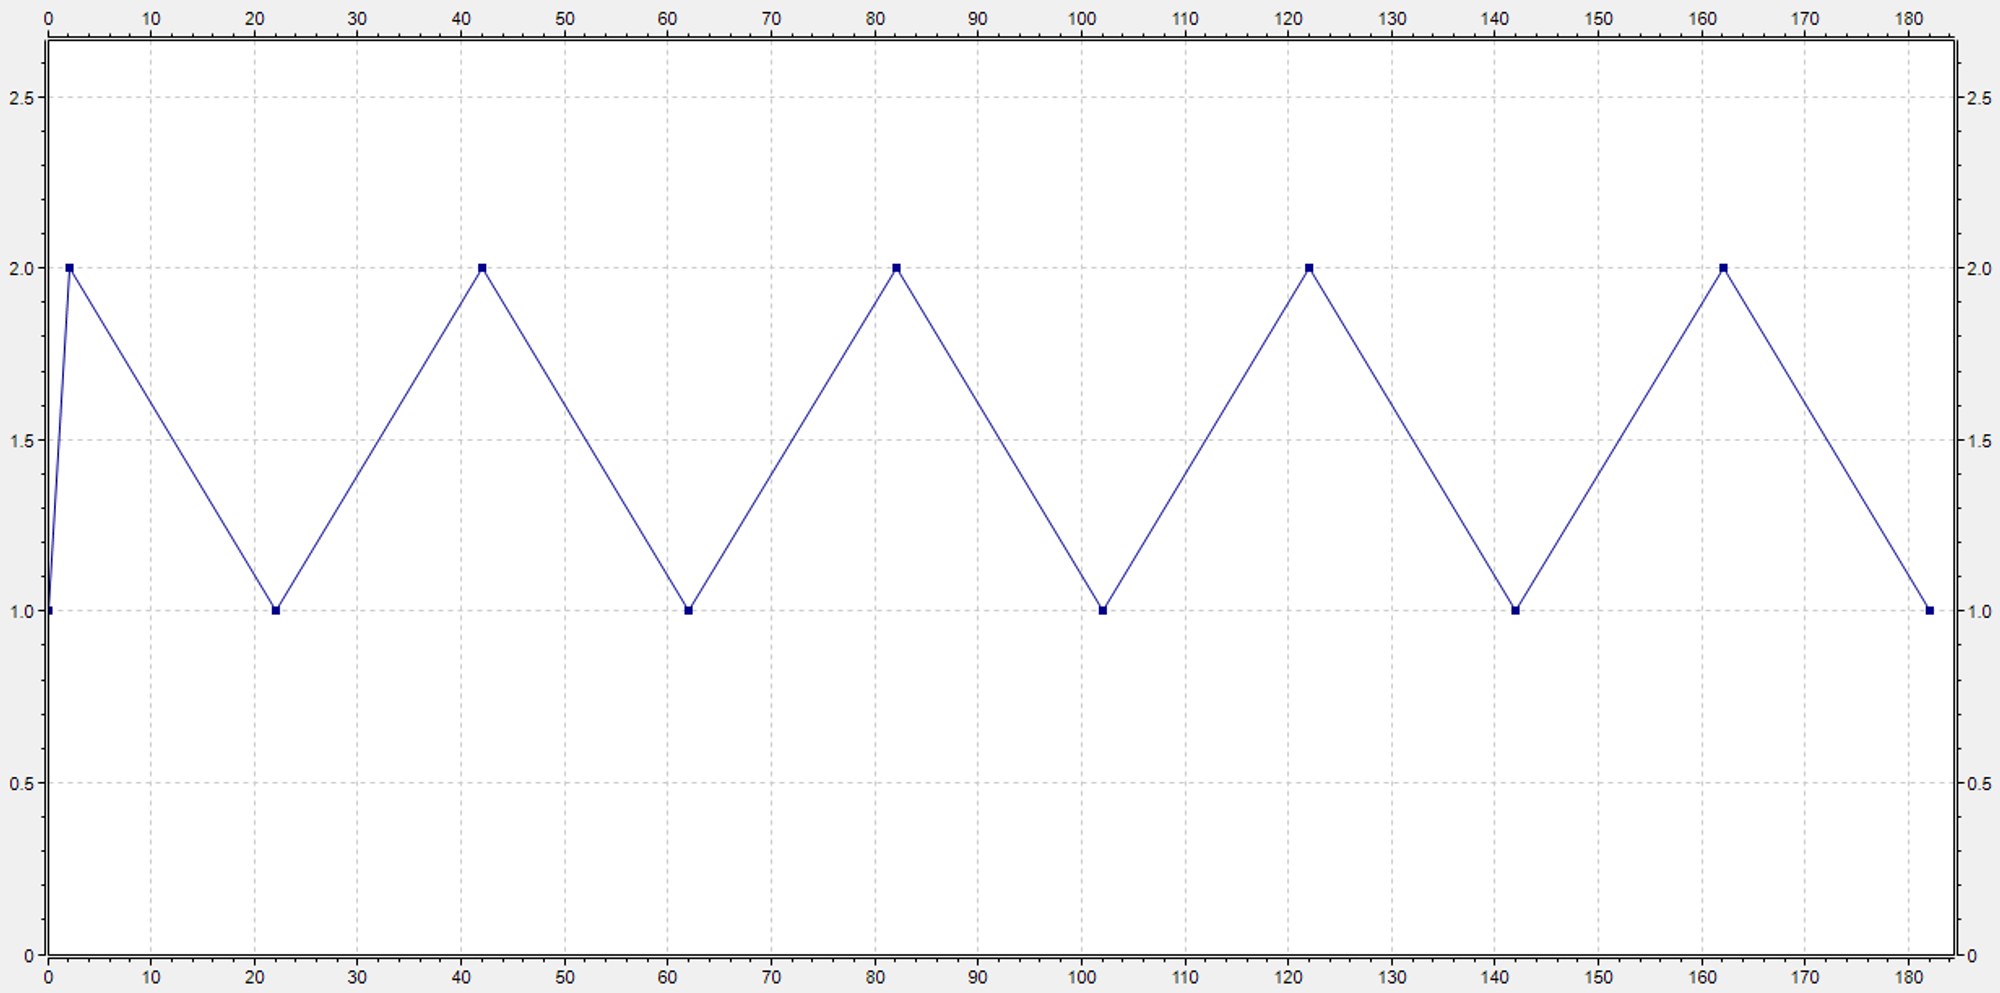
\includegraphics[width=.68\textwidth]{image/week11/2-1-3.png}
	        \caption{\footnotesize
	        experiment 2-1, sevingCell}
	        \vspace{-10pt}
        \end{figure}
    \subsubsection*{2. 1. 3 Discussion}
    \vspace{-3mm}
        단말이 이동함에 따라 단말 ue11의 servingCell이 eNodeB1과 eNodeB2로 계속해서 바뀌는 handover를 확인할 수 있다. 
%%%%%%%%%%%%%%%%%%%%%%%%%%%%%%%%%%%%%%%%%%%%%
\subsection*{Experiment 2-2}
    \subsubsection*{2. 2. 1 Code}
    \vspace{-3mm}
    실험 2-1과 같은 코드에 다음의 부분을 추가로 변경했다.
            \vspace{-2mm}
            \begin{listing}[h!]
            \inputminted[framerule = 1pt,framesep = 2mm , frame = lines, fontsize=\footnotesize]{c}{./code/week11/Experiment_02/omnet4.cpp}
            \vspace{-3mm}
            \caption{\footnotesize experiment 2-2, omnetpp.ini}
            \end{listing}
            \vspace{-6mm}
    \subsubsection*{2. 2. 2 Simulation}
    \vspace{-3mm}
        실험 2-1과 같은 네트워크에서 단말 ue11과 ue12의 이동속도를 10mps에서 20mps로 2배 증가시켰다. \\
        시뮬레이션 진행중 단말의 이동이 나타나도록 화면녹화 screenshot 영상을 촬영해 youtube에 업로드하였다. 해당 영상은 아래의 링크를 클릭해 이동이 가능하다.
        \vspace{-10mm}
            \begin{center}
                \item \href{https://www.youtube.com/watch?v=caP-YgTERbA&ab_channel=anamnesis}
            	{Youtube link of Week11 Experiment 2-2 Simulation Results Screenshot Video}
            \end{center}
        \vspace{-6mm}
        \begin{figure}[h!]
            \centering
            \subfloat[screenshot 1]{
                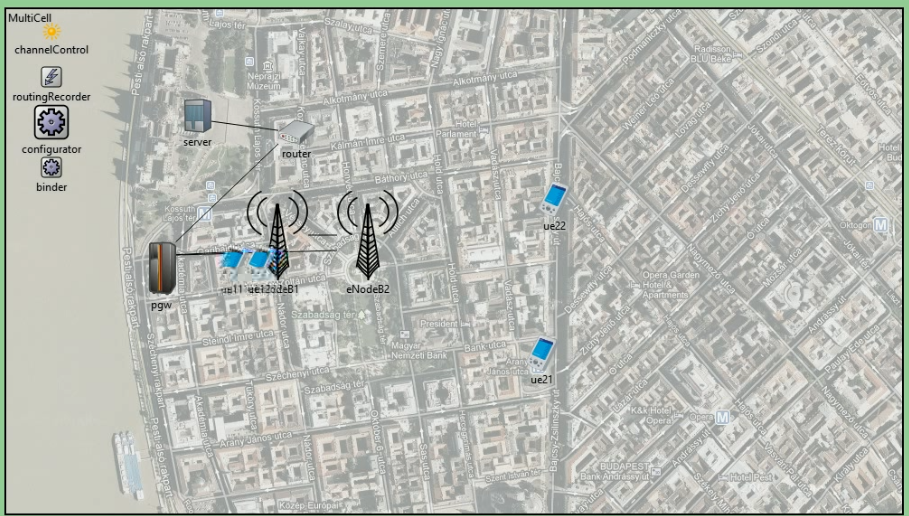
\includegraphics[width=0.45\textwidth]{image/week11/2-2-1.png}
            }\hspace{3mm}
            \subfloat[screenshot 2]{
                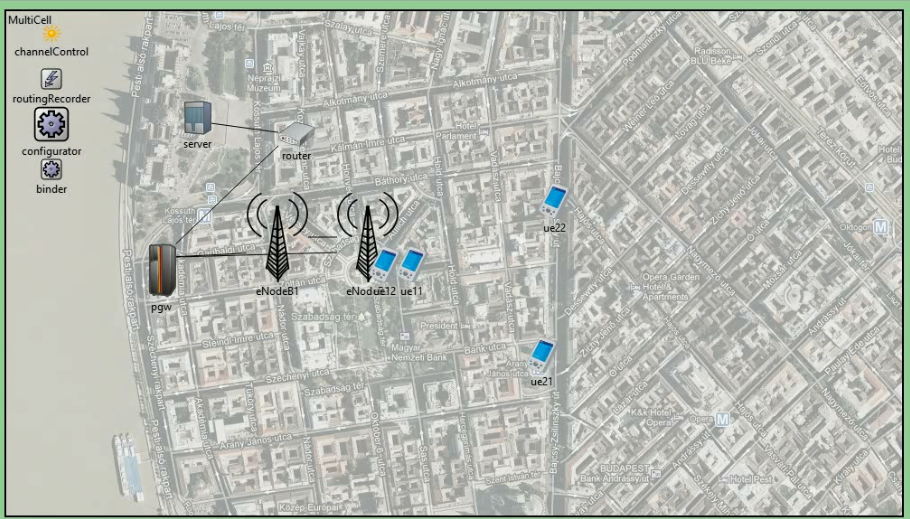
\includegraphics[width=0.45\textwidth]{image/week11/2-2-2.png}
            }\hspace{3mm}
            \caption{experiment 2-1, network simulation}
        \end{figure}
        시뮬레이션 종료 후 생성된 벡터 데이터 중에서 시간에 따른 단말 ue11의 servingCell 값을 확인했다.
        \begin{figure}[!h]\centering 
	        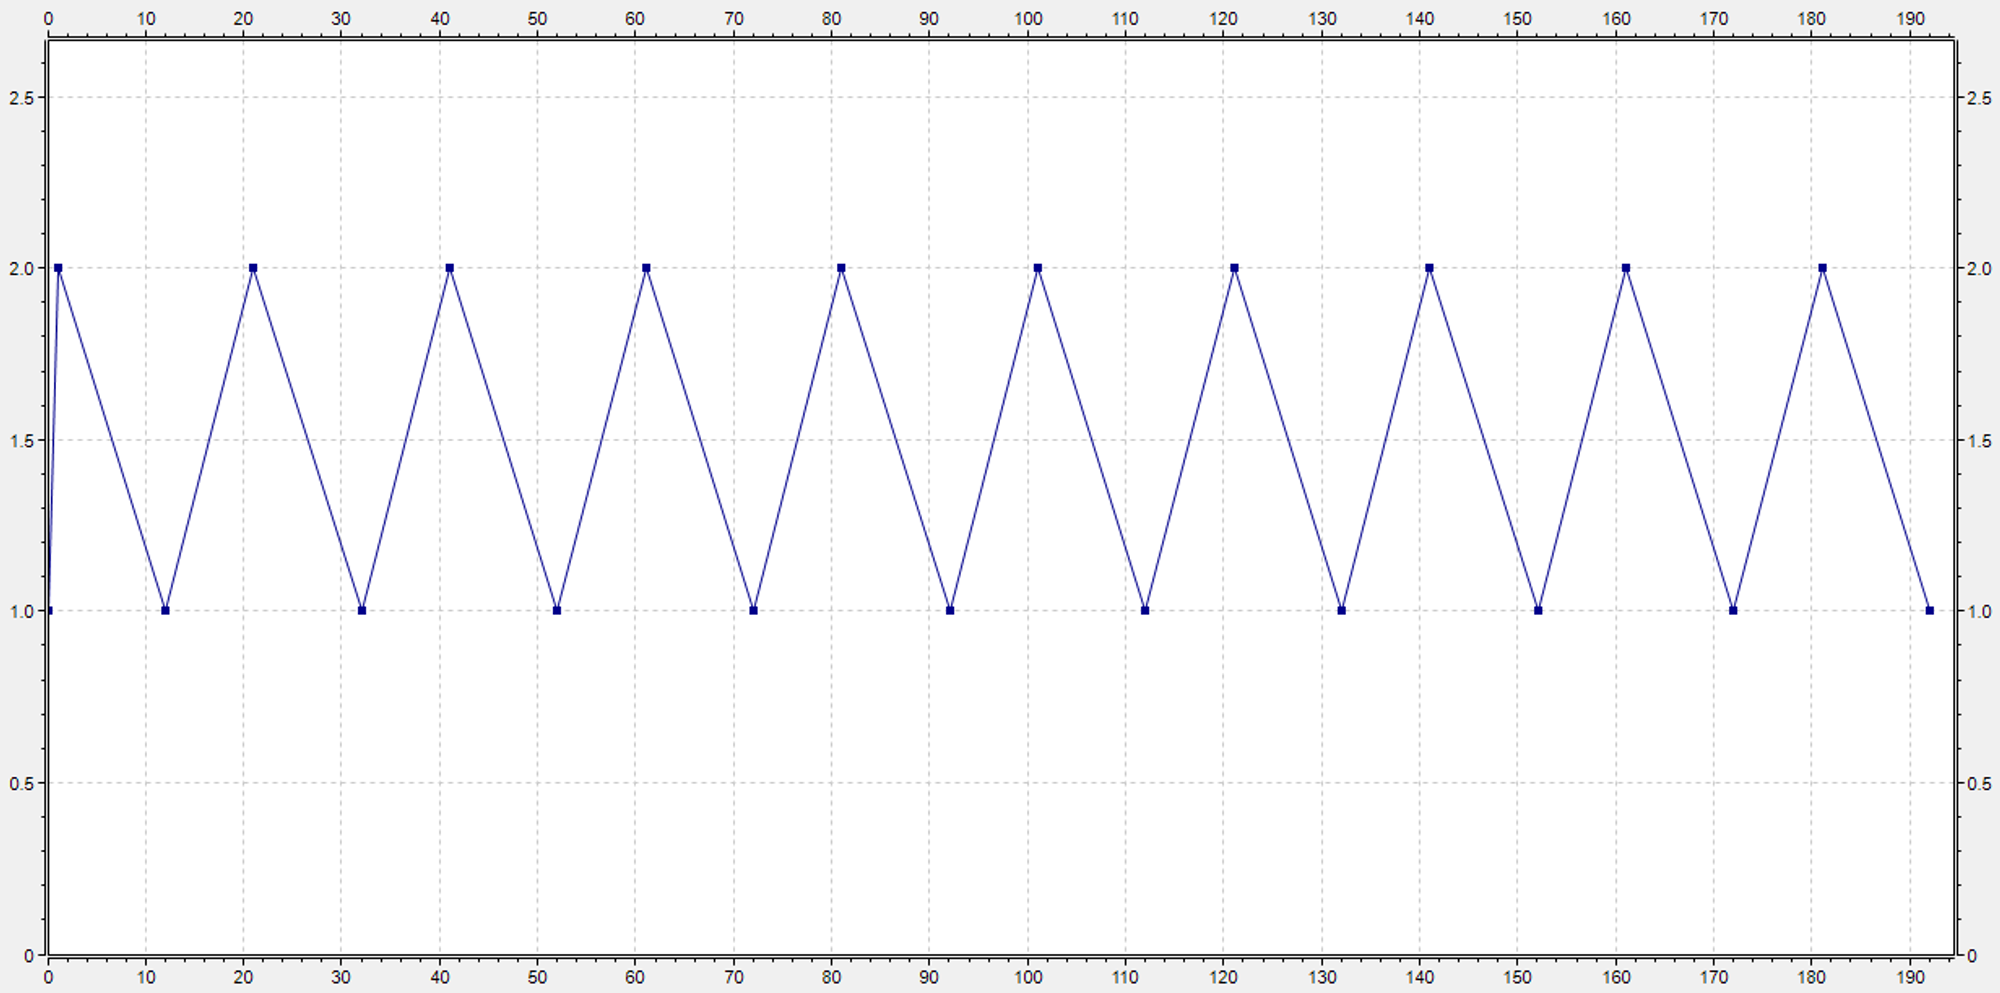
\includegraphics[width=.68\textwidth]{image/week11/2-2-3.png}
	        \caption{\footnotesize
	        experiment 2-2, sevingCell}
	        \vspace{-10pt}
        \end{figure}
    \subsubsection*{2. 2. 3 Discussion}
    \vspace{-3mm}
        단말이 이동함에 따라 단말 ue11의 servingCell이 eNodeB1과 eNodeB2로 계속해서 바뀌는 handover를 확인할 수 있다. 실험 2-1과 비교할 때, 단말의 이동 속도 증가로 servingCell이 바뀌는 주기가 2배 더 빨라진 것을 확인할 수 있다.